\documentclass{VUMIFPSkursinis}
\usepackage{algorithmicx}
\usepackage{algorithm}
\usepackage{algpseudocode}
\usepackage{amsfonts}
\usepackage{amsmath}
\usepackage{array}
\usepackage{bm}
\usepackage{caption}
\usepackage{color}
\usepackage{float}
\usepackage{graphicx}
\usepackage{listings}
\usepackage{longtable}
\usepackage{subfig}
\usepackage{wrapfig}
\usepackage{enumitem}

\usepackage[tableposition=top]{caption}


%PAKEISTA, tarpai tarp sąrašo elementų
\setitemize{noitemsep,topsep=0pt,parsep=0pt,partopsep=0pt}
\setenumerate{noitemsep,topsep=0pt,parsep=0pt,partopsep=0pt}

\newcolumntype{L}[1]{>{\raggedright\let\newline\\\arraybackslash\hspace{0pt}}m{#1}}
\newcolumntype{C}[1]{>{\centering\let\newline\\\arraybackslash\hspace{0pt}}m{#1}}
\newcolumntype{R}[1]{>{\raggedleft\let\newline\\\arraybackslash\hspace{0pt}}m{#1}}

% Titulinio aprašas
\university{Vilniaus universitetas}
\faculty{Matematikos ir informatikos fakultetas}
\department{Programų sistemų katedra}
\papertype{Kursinis darbas}
\title{Blokų grandinės technologija. Išmaniųjų kontraktų platformos}
\titleineng{Blockchain technology. Smart Contract platforms}
\status{3 kurso 3 grupės studentas}
\author{Gediminas Krasauskas}
\supervisor{prof. dr. Saulius Minkevičius}
\date{Vilnius – \the\year}

% Nustatymai
% \setmainfont{Palemonas}   % Pakeisti teksto šriftą į Palemonas (turi būti įdiegtas sistemoje)
\bibliography{bibliografija}

\begin{document}
\maketitle

\tableofcontents

\sectionnonum{Įvadas}
Pastaraisiais metais užsienio ir Lietuvos visuomenės žiniasklaidoje, socialiniuose tinkluose daug atgarsio bei kontroversijos sulaukia blokų grandinė, jos pagrindu kuriami startuoliai, išmanieji kontraktai, kriptovaliutos. Tačiau dėl masinės manijos ir naujovių rinkoje ne visi supranta šių terminų ir technologijų esmės, veikimo principų. Todėl matome susiskaldymą: vieni mano, kad blokų grandinė yra ateitis, kuri pakeis mūsų pasaulį \cite{crosby2016blockchain}, o kiti mato technologijos panašumų į jau matytus istorinius technologinius burbulus \cite{folkinshteyn2015tale}. Nors rinka ir yra nepastovi – populiariausios kriptovaliutos Bitkoino vertė 2017 metais pasiekė beveik 20 tūkst. JAV dolerių kainą, o 2018 m. pirmame ketvirtyje pastebimas vertės nuosmukis \cite{hale2018futures} – technologijos aktualumą ir panaudojimo galimybes būtų sunku paneigti.

Vienas pagrindinių tikslų, kurių siekia verslas pasauliui modernėjant, yra palengvinti kasdienius procesus, juos automatizuoti, sumažinti žmogiškųjų išteklių, skirtų atlikti užduotį, kiekį. Viena esminių sričių, kur tai atsipirktų ir atneštų pridėtinę vertę, yra finansai ir paslaugos: bankai, draudimas, nekilnojamasis turtas, akcijų biržos ir dar daug kitų.

Jau daug metų turime nusistovėjusią sistemą, kai norint pervesti pinigus kitam žmogui, turime pasikliauti tarpininkais – bankais. Tai bankai yra atsakingi už transakcijų patikimumą, mūsų pinigų ir asmeninių duomenų saugumą. To kaina – mokesčiai už kiekvieną bankinį pavedimą, pinigų išsigryninimą, banko sąskaitos palaikymą ir t.t. Tačiau toks modelis vyrauja ne tik su bankais, bet ir su kiekviena sritimi, kuri reikalauja kažkokio tarpininko. Būtų idealu, jei pinigų laikymas, paslaugų teikimas vyktų decentralizuotai ir automatizuotai, t.y. be jokių tarpininkų ir atskirų žmonių įsikišimo, tarsi viena didelė ekosistema, kuri priklausytų nuo visų ekosistemos dalyvių. 

Ir tai tampa vis labiau aktualu šiandien, kai stebime modernėjančią visuomenę, augantį kompiuterinį raštingumą, o išmanieji telefonai tampa galingiausiu įrankiu žmogaus gyvenime. Programų sistemų inžinieriai deda visas pastangas, kad paslaugos ir atsiskaitymai pilnai persikeltų į internetą ir taptų maksimaliai automatizuoti. Ieškomi sprendimai gaišaties, išlaidų ir klaidų veiksnių, kuriuos lemia žmogiškieji ištekliai, sumažinimui. Tuo tarpu vartotojams didesnę reikšmę vis labiau įgyja asmens duomenų apsauga, pasirinkimo įvairovė, greitis, paprastumas.

Blokų grandinės technologija, išmaniųjų kontraktų platformos panašu ir bus tai, kas patenkins šiuos poreikius bei išspręs minėtas problemas. Tačiau šios technologijos dar labai jaunos ir nespėjusios nusistovėti, joms trūksta pilnesnės ir užbaigtos infrastruktūros išvystymo. Jau ilgą laiką rinkoje galėjome matyti vieną įsitvirtinusį žaidėją – Ethereum, tačiau pastaruoju metu stebime ir daugiau panašių projektų startavimų, tokių kaip EOS, atnešančių naujų idėjų ir ilgojoje perspektyvoje galinčių nukonkuruoti Ethereum.

Taigi, šio darbo tikslas – ištirti blokų grandinės ir išmaniųjų kontraktų technologijas, palyginti EOS ir Ethereum išmaniųjų kontraktų platformas. Šiam tikslui pasiekti keliami tokie uždaviniai:


\begin{itemize}
    \item Išsiaiškinti blokų grandinės, išmaniųjų kontraktų ir kitas svarbias sąvokas, jų veikimo principus bei modelius.
    \item Apžvelgti Ethereum išmaniųjų kontraktų platformą.
    \item Apžvelgti EOS išmaniųjų kontraktų platformą.
    \item Ištirti Ethereum ir EOS išmaniųjų kontraktų platformų skirtumus jas palyginant.
\end{itemize}

\section{Blokų grandinė}
Blokų grandinė (angl. \textit{Blockchain}) – tai nuolat augantis blokais sujungtas sąrašas, kuris yra apsaugotas naudojant kriptografijos metodus. Blokų grandinės kontekste blokas yra įrašų (dažniausiai transakcijų) ir atributų, būtinų blokų grandinei sėkmingai funkcionuoti, visuma.

Nors iš šiandienos aktualijų ir atrodytų, kad technologija yra šviežia, tačiau jos užuomazgas buvo galima aptikti dar 1978 metais, kai buvo patentuotas blokų surišimas ieškant klaidų žinučių patvirtinimuose ir perdavimuose \cite{ehrsam1978message}. Tačiau blokų grandinės technologija labiausiai išpopuliarėjo ir įgavo apčiuopiamą pritaikymą tik po 3 dešimtmečių, 2008 metais, kuomet Satoshi Nakamoto pristatė pirmąją pasaulyje blokų grandinę su funkcionuojančia kriptovaliuta Bitkoinu (angl. \textit{Bitcoin}) \cite{nakamoto2008bitcoin}. Taigi galima būtų teigti, kad blokų grandinė nebuvo išrasta, o labiau evoliucionavo laikui bėgant.

\subsection{Verslo tinklų modeliai}
Standartiniame verslo tinklo modelyje kiekviena šalis saugo savo įrašus, nuosavybę (žr. Priedas nr. 1). Šis modelis turi nemažai trūkumų. Vienas jų – atliekant transakcijas arba bendraujant su kitomis šalimis yra įtraukiami tarpininkai, kuriems už teikiamas paslaugas ir prisiimtą atsakomybę reikia mokėti mokestį. Dar vienas tarpininkų trūkumas – procesas užsitęsia dėl įsipareigojimų vykdymo, įrašų kopijų darymo, papildomų saugumo užtikrinimo operacijų ir t.t. Taip pat šis modelis yra lengvai pažeidžiamas. Pavyzdžiui, jei centrinė sistema, tarkime bankas, susikompromituotų dėl sukčiavimo atvejų, kibernetinių atakų ar paprasčiausių žmogiškųjų klaidų, pasekmes jaustų visi tinklo nariai. Galiausiai, toks modelis sąlygoja potencialias cenzūros, asmens duomenų manipuliacijos, monopolio rizikas \cite{catalini2017some}.

Tuo tarpu verslo tinklo modelyje, kuris naudoja blokų grandinės technologiją (žr. Priedas nr. 2), visi nariai turi visas bendro tinklo įrašų kopijas ir gali būti tiek prenumeratoriai, tiek skelbėjai vienu metu. Kiekviena šalis gali atlikti tiesioginius sandorius su kitoms šalims. Visi duomenys yra sinchronizuojami tinkle visiems naudotojams realiu laiku.

Kitaip tariant, blokų grandinės tinklas yra ekonomiškesnis ir našesnis, nes yra pašalinamas tarpininkų poreikis. Taip pat jis patikimesnis, nes transakcijos yra saugios, patvirtinamos ir verifikuojamos, o visi transakcijų įrašai yra atvirai prieinami visiems tinklo naudotojams \cite{chiu2017economics}.

\subsection{Pagrindinės charakteristikos}
Blokų grandinės tinklui galima priskirti kelias pagrindines charakteristikas \cite{deloite2017}:
\begin{itemize}
    \item \textbf{Paremtas konsensusu}. Tam, kad transakcija blokų grandinėje būtų įvykdyta, visi arba dauguma tinklo narių privalo vieningai sutikti su transakcijos tinkamumu.
    \item \textbf{Aiški kilmė}. Visi tinklo nariai turi žinoti iš kur kiekvieno nario turima nuosavybė atsirado ir kaip nuosavybės autorystė keitėsi laikui bėgant.
    \item \textbf{Paskirstyta saugykla}. Identiškos duomenų kopijos yra saugomos pas visus blokų grandinės narius. Todėl jei bent vienas tinklo narys susikompromituoja, likę nariai toliau sklandžiai dalyvauja blokų grandinės veikime. Kiekvienas narys turi teisę dalyvauti patvirtinant transakcijas arba pats bendrauti su kitais nariais vykdant transakcijas be papildomų tarpininkų.
    \item \textbf{Pilnai skaitmeninė}. Visi duomenys blokų grandinėje yra skaitmeninėje formoje. Šitaip yra pašalinamas popierizmas ir galimas informacijos klastojimas.
    \item \textbf{Naudojami kriptografijos elementai}. Sukurti blokai yra įrašomi į blokų grandinę naudojant kriptografijos moksle taikomus metodus. Tai reiškia, kad ištrinti, gadinti arba klastoti bloką, įrašytą į blokų grandinę, yra be galo sunku – nei vienas tinklo narys neturi teisės savavališkai to daryti. Šitaip atsiranda pagrįsta skaitmeninė nuosavybė, aukšto lygio patvarumas ir pasitikėjimas. 
\end{itemize}

\subsection{Veikimo principas}
Blokų grandinės pavadinimas atsiranda iš to, kaip technologija veikia (1 pav.). Visi transakcijų duomenys – įrašai – yra saugomi blokuose. Kiekvienas blokas savyje saugo tam tikrus atributus: bloko numerį, bloko maišos reikšmę (angl. \textit{Hash}), ankstesniojo bloko maišos reikšmę, laiko žymę (angl. \textit{Timestamp}) ir tam tikrą kiekį transakcijų. 

Bloko maišos reikšmė – tai unikalus bloko identifikatorius. Kiekviename bloke saugoma ankstesniojo bloko maišos reikšmė leidžia einamąjį bloką sujungti su prieš jį esančiu bloku. Šitokiu būdu yra auginama grandinė, tačiau taip pat yra apsisaugoma nuo blokų modifikavimo arba naujų blokų įterpimo tarp dviejų jau egzistuojančių blokų. Kaskart prie blokų grandinės prijungus naują bloką, visa sistema pasidaro patvaresnė ir saugesnė \cite{chiu2017economics}.

Kiekviena bloke užfiksuojama transakcija paprastai turi savo laiko žymę, siuntėją, gavėją ir transakcijos metu perleistą nuosavybę. Tada transakcijos duomenys paverčiami į maišos reikšmę. Svarbu paminėti tai, kad blokų grandinės pritaikymų yra labai daug ir nuo kiekvieno pritaikymo blokų sudėtis gali skirtis, tačiau pagrindiniai principai lieka tokie patys.

\begin{figure}[H]
    \centering
    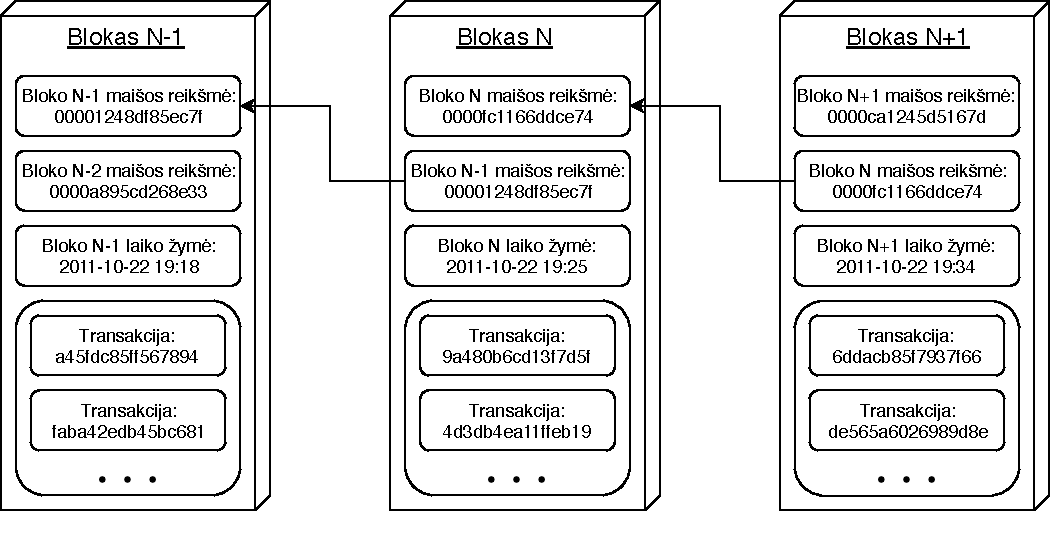
\includegraphics[scale=0.85]{img/pav-block-chain.pdf}
    \caption{Blokų grandinės veikimo modelis}
    \label{img:pav-block-chain}
\end{figure}

\section{Išmanieji kontraktai}
Išmanieji kontraktai (angl. \textit{Smart Contracts}) yra vienas praktiškiausių blokų grandinės panaudojimo būdų. Pirmą kartą išmaniųjų kontraktų terminas buvo panaudotas 1994 metais, mokslininko Nick Szabo \cite{szabo1994smart}. Išmanųjį kontraktą būtų galima apibrėžti kaip protokolą, programą, kuri įgyvendina automatinius skaitmeninės nuosavybės pervedimus tarp skirtingų šalių remiantis bendrai sutartomis ir apibrėžtomis taisyklėmis.

\subsection{Pagrindinės charakteristikos}
Išmanieji kontraktai yra labai panašūs į realaus pasaulio kontraktus. Tačiau galime išskirti kelias esmines savybes, kurios išmaniuosius kontraktus padaro unikalias:
\begin{itemize}
    \item \textbf{Pilnai automatizuoti}. Kadangi išmanusis kontraktas yra programinis kodas, tai jo vykdymas nereikalauja žmonių įsikišimo. Esant tam tikroms sąlygoms ir aplinkybėms, kodas pats pasileidžia ir įvykdo tai, ką jis yra užprogramuotas daryti.
    \item \textbf{Kontrakto stabilumas}. Išmanieji kontraktai yra talpinami blokų grandinėje. Vien tai išmaniesiems kontraktams suteikia daug savybių, kuriomis pasižymi ir blokų grandinė. Viena esminių yra ta, kad išmanusis kontraktas yra stabilus – niekas negali jo redaguoti arba ištrinti, todėl sukuriamas pasitikėjimas tarp visų tinklo narių.
    \item \textbf{Pilnai skaitmeniniai}. Visi išmanieji kontraktai yra patalpinti blokų grandinėje, todėl yra apsieinama be popierizmo, notarų arba raštiškų parašų – tai leidžia naudotis kontraktais neišeinant iš namų.
    \item \textbf{Atvirumas}. Visi blokų grandinės tinklo naudotojai gali pamatyti visas išmaniojo kontrakto detales, t.y. programinį kodą. Nėra jokių paslėptų taisyklių arba įsipareigojimų mažomis raidėmis.
    \item \textbf{Paprasta ir greita}. Viskas, ką reikia padaryti blokų grandinės tinklo naudotojui – tai suaktyvinti kontraktą arba leisti kontraktui aktyvuotis pačiam, esant tam tikroms sąlygoms, aplinkybėms. Išmanusis kontraktas įsipareigojimus įvykdys valandų arba minučių bėgyje, priklausomai nuo išmaniųjų kontraktų platformos.
\end{itemize}

\subsection{Svarbiausios sąvokos}
Tam, kad geriau suprastume, kaip veikia išmanieji kontraktai, turime susipažinti su keliomis sąvokomis, kurios bus paaiškintos toliau esančiuose poskyriuose. 

\subsubsection{Kriptovaliutos}
Kriptovaliuta (angl. \textit{Cryptocurrency}) – tai skaitmeninė, virtuali valiuta, leidžianti atlikti tiesioginius mokėjimus tarp blokų grandinės tinklo naudotojų, pašalinant tarpininkų būtinybę. Pati pirmoji kriptovaliuta buvo sukurta 2009 metais ir buvo pavadinta Bitkoinu. Remiantis Jan Lansky moksliniu straipsniu, kriptovaliuta yra sistema, kuri atitinka 6 sąlygas \cite{lansky2018possible}:
\begin{enumerate}
    \item Sistemai yra nereikalinga centrinė institucija, kuri reguliuotų kriptovaliutų vienetų išdavimą ir auditą.
    \item Sistema saugo ir nuolat pildo kriptovaliutos vienetų ir jų nuosavybės žurnalą. 
    \item Sistema apibrėžia, ar galima sukurti naujus kriptovaliutos vienetus. Jei galima sukurti naujus kriptovaliutos vienetus, sistema apibrėžia jų atsiradimo aplinkybes ir tai, kaip nustatyti šių naujų kriptovaliutos vienetų nuosavybę.
    \item Kriptovaliutos vienetų nuosavybės teisė gali būti įrodyta tik kriptografiškai.
    \item Sistema leidžia atlikti sandorius, kuriuose perleidžiama kriptografinių vienetų nuosavybė. Sandorio patvirtinimą gali išduoti tik ta šalis, kuri įrodo dabartinę šių kriptovaliutos vienetų nuosavybę.
    \item Jei tuo pačiu metu pateikiami du skirtingi nurodymai dėl tų pačių kriptovaliutų vienetų nuosavybės keitimo, sistema įvykdo tik vieną iš jų.
\end{enumerate}

\subsubsection{Kriptovaliutų piniginės}
Dar vienas svarbus terminas – kriptovaliutos piniginė (angl. \textit{Cryptocurrency Wallet}). Ši piniginė – tai banko sąskaitos analogija, kuri blokų grandinės kontekste saugo kriptovaliutų vienetus. Kriptovaliutos piniginė savyje taip pat saugo privatų ir viešą raktus, kuriuos naudoja tiek gaunant, tiek siunčiant kriptovaliutos vienetus į kitas pinigines \cite{herbert2015novel}. 

\subsubsection{Decentralizuotos programėlės}
Decentralizuotos programėlės (DApps) – tai paprasčiausios programėlės, išsiskiriančios savo vienu požymiu: jos kertinis vidinio programavimo (angl. \textit{Backend}) funkcionalumas, išmanusis kontraktas, yra patalpintas ne nuotoliniame serveryje, o blokų grandinėje \cite{jiao2018auction}. Tai reiškia, kad programėlė nėra valdoma korporacijos arba vieno žmogaus, o tuo pačiu yra atviro kodo. Kiekviena DApp pagal poreikį gali turėti savo vietinę valiutą, su kuria galima atsiskaityti už paslaugas. Tai yra pasiekiama žetonų (angl. \textit{Tokens}) dėka.

\subsubsection{Žetonai}
Žetonai yra reikalingi tam, kad decentralizuotomis programėlėmis vartotojams būtų galima naudotis greičiau, pigiau ir paprasčiau. Žetonai yra išduodami naudojant tokį standartinį modelį \cite{catalini2018initial}:
\begin{itemize}
    \item Decentralizuotos programėlės kūrėjai paskelbia pirminį kriptovaliutos siūlymą (angl. \textit{Initial Coin Offering}) – ICO, kuris turi apibrėžtą išmanųjį kontraktą, nurodantį projekto sėkmės taisykles ir žetonų platinimo detales. Pavyzdžiui, projekto sėkmės taisyklė gali būti tokia, kad per mėnesį nuo decentralizuotos programėlės sukūrimo turi būti nupirkta žetonų už milijoną eurų. Jeigu suma nebus pasiekta per mėnesį, pirminis kriptovaliutų siūlymas žlunga.
    \item Fiziniai arba juridiniai asmenys, susidomėję decentralizuota programėle ir tikintys jų vertės augimu ateityje, investuoja į decentralizuotą aplikaciją, keisdami kriptovaliutas arba realius pinigus į siūlomus žetonus.
    \item Jeigu per pirminio kriptovaliutų siūlymo laikotarpį tikslai nėra pasiekiami, išmanusis kontraktas pasirūpina, kad visi asmenų, kurie investavo į decentralizuotą programėlę, kriptovaliutos arba pinigai yra grąžinami. Jeigu tikslai pasiekiami, žetonai tampa jų pirkėjų nuosavybe.
\end{itemize}
Paprastai žetonai yra skirstomi į 4 kategorijas \cite{pietrewicz2017emerging}:
\begin{itemize}
    \item \textbf{Tradiciniai turto žetonai} (angl. \textit{Traditional Asset Tokens}). Šie žetonai nurodo tradicinio turto, tokio kaip nekilnojamasis turtas, nuosavybę. Šiuo metu tai rečiausiai pasitaikantys žetonai.
    \item \textbf{Naudojimo žetonai} (angl. \textit{Usage Tokens}). Šie žetonai reikalaingi siekiant prieigos prie išmaniųjų programėlių tiekiamų paslaugų. Tai bene labiausiai paplitusi žetonų kategorija.
    \item \textbf{Darbiniai žetonai} (angl. \textit{Work Tokens}). Tai žetonai, kurių savininkams yra suteikiamas decentralizuotos programėlės akcininko statusas. Tai leidžia žetonų savininkui turėti balso teisę sprendžiant, pavyzdžiui, DApp tolimesnį vystymosi planą.
    \item \textbf{Hibridiniai žetonai} (angl. \textit{Hybrid Tokens}). Šie žetonai paprastai yra naudojimo ir darbinių žetonų junginys.
\end{itemize}

\subsection{Išmaniojo kontrakto sandara}
Išmanusis kontraktas savo sandara yra labai panašus į kriptovaliutų piniginę. Jį sudaro \cite{delmolino2016step}:
\begin{itemize}
    \item \textbf{Adresas}. Tai viešas kontrakto identifikatorius, kuris leidžia tinklo naudotojams siųsti kriptovaliutų vienetus į  kontrakto sąskaitą.
    \item \textbf{Sąskaitos likutis}. Tai kriptovaliutos vienetai, kuriuos turi ir valdo išmanusis kontraktas.
    \item \textbf{Būsena}. Tai esama visų kintamųjų, deklaruotų išmaniajame kontrakte, būsena. Tai labai panašu į objektiškai orientuotas programavimo kalbas, kai sukuriant objektą yra sukuriamos ir pradinės to objekto atributų būsenos, kurios kinta programos eigoje. 
    \item \textbf{Kodas}. Tai kodas, kuris yra įvykdomas sukuriant kontraktą bei metodų rinkinys, kuriuos galima iškviesti pagal poreikį – visai kaip ir objektų metodai objektiškai orientuotose programavimo kalbose.
\end{itemize}

\subsection{Veikimo principas}
Yra sukurta daug išmaniųjų kontraktų platformų, o pačius kontraktus galima suprogramuoti įvairiomis programavimo kalbomis. Nepaisant šios įvairovės, išmaniųjų kontraktų veikimo principas nesiskiria. Kaip jau žinome, išmanusis kontraktas yra ne kas kita, kaip programinis kodas. Supaprastinus modelį, galime sakyti, kad esant įvykiui X, išmanusis kontraktas atliks veiksmų seką, kurio galutinis rezultatas bus Y.

X gali būti bet koks įvykis, kurį galima užfiksuoti programiniu būdu. Pavyzdžiui: drėgmės jutikliai užfiksuoja sausrą, kuri tęsiasi 2 savaites ir duomenis, įrodančius stichinę anomaliją, patalpina į blokų grandinę. Y turi būti įvykis, kurį įmanoma užprogramuoti ir įvykdyti programiniu būdu. šiuo atveju galima įgalinti išmaniuosius kontraktus. Galėtume sukurti tokį kontraktą, kuris apdraustų ūkininkų pasėlius. 

Turėtume apibrėžti tokias kontrakto sąlygas: 
\begin{enumerate}
    \item Ūkininkas sutinka iš savo kriptovaliutų piniginės kiekvieną mėnesį automatiškai pervesti tam tikrą kriptovaliutos vienetų kiekį į išmaniojo kontrakto paskyrą. Šitaip ūkininkas apdraudžia savo ūkį.
    \item Drėgmės jutikliams užfiksavus sausrą ir tai patvirtinančius duomenis patalpinus į blokų grandinę, išmaniojo kontrakto paskyra iškart automatiškai perveda tam tikrą kriptovaliutos vienetų kiekį į apsidraudusių ūkininkų kriptovaliutų pinigines.
    \item Kiekviena šalis turi turėti reikiamą kiekį kriptovaliutos vienetų savo sąskaitoje. Priešingu atveju sandoris yra nutraukiamas arba nepradedamas.
    \item Kiekviena šalis gali bet kuriuo momentu nutraukti sutartį.
    \item Abi šalys privalo sutikti su visomis kontrakto sąlygomis.
\end{enumerate}

Išmanieji kontraktai dirba su 2 rūšių paskyromis: tai naudotojų paskyros, kurias gali valdyti tiek fiziniai, tiek juridiniai asmenys, ir kontraktų paskyros, kurių nevaldo niekas, išskyrus pats kontraktas. Nors prieš tai pateiktame pavyzdyje nagrinėjome atvejį, kuriame įvyksta sandoris tarp naudotojo paskyros ir kontrakto paskyros, sandorių šalys gali varijuoti. 

Iš viso galimos 4 sandorių variacijos:
\begin{itemize}
    \item Naudotojo paskyra atlieka sandorį su kito naudotojo paskyra.
    \item Naudotojo paskyra atlieka sandorį su kontrakto paskyra.
    \item Kontrakto paskyra atlieka sandorį su naudotojo paskyra.
    \item Kontrakto paskyra atlieka sandorį su kito kontrakto arba savo paskyra.
\end{itemize}

\section{Išmaniųjų kontraktų platformos}
Išmanieji kontraktai siūlo nemažai galimybių, tačiau turi egzistuoti speciali platforma, kuri leistų jiems funkcionuoti blokų grandinėje. Šiuo metu egzistuoja daug išmaniųjų kontraktų platformų, tačiau nagrinėsime dvi populiariausias platformas. Tai Ethereum ir EOS.

\subsection{Ethereum išmaniųjų kontraktų platforma}
Ethereum – tai atviro kodo blokų grandinės technologija paremta platforma, decentralizuota operacinė sistema, palaikanti išmaniųjų kontraktų funkcionalumą. Ethereum technologiją pristatė Vitalik Buterin 2013 metais, o jau 2015 liepos 30 d. platforma buvo oficialiai išleista ir prieinama naudotis visiems. 

\subsubsection{Ethereum kriptovaliuta Ether}
Ethereum kūrėjų komanda pristatė ne tik platformą, įgalinančią išmaniųjų kontraktų veikimą ir decentralizuotų aplikacijų kūrimą, bet ir sukūrė savo atskirą kriptovaliutą – Ether (ETH). Nors valiuta ir turėjo lėtą startą, tačiau per 2017 metų laikotarpį Ether akcijos išaugo 13000\% ir šiuo metu užtikrintai užima 2 vietą pagal visos vertės dalį kriptovaliutų rinkoje, atsiliekanti tik nuo Bitkoino\footnote{https://coinmarketcap.com. Tikrinta 2018-06-17}. ETH kriptovaliutos pagrindinė paskirtis – apmokėti kompiuterinių skaičiavimų sąnaudas ir transakcijų mokesčius.

\subsubsection{Ethereum ERC20 žetonai}
Ne paslaptis, kad prie Ether sėkmės ženkliai prisidėjo spartus decentralizuotų aplikacijų kūrimas, kuris padidino šios kriptovaliutos paklausą. Tam tikroms decentralizuotoms programėlėms egzistuoja poreikis turėti savo žetonus vietoje to, kad naudotojas atsiskaitytų už paslaugas tiesiogiai ETH kriptovaliuta. Tai suteikia papildomą komfortą, greitumą ir paprastumą sistemų naudotojams. 

Ethereum platforma pateikia specialų žetonų standartą, pavadinimu ERC20. ERC20 žetonai – tai standartas, rinkinys funkcijų, kuriuos turi atitikti žetonai. Jeigu žetonas atitinka ERC20 reikalavimus, tai yra ERC20 žetonas. Nors ir nėra privaloma, tačiau decentralizuotų aplikacijų kūrėjams Ethereum platformoje yra rekomenduojama laikytis standarto, nes tai užtikrina, kad jų žetonai gali sąveikauti su įvairiomis kriptovaliutų piniginėmis, keityklomis (angl. \textit{Exchanges}) ir išmaniaisiais kontraktais išvengiant problemų dėl nesuderinamumo. 

Bendras standartas labai palengvino programuotojų darbą. Kol neegzistavo šis standartas, visi žetonų kūrėjai privalėjo kurti savo standartų versijas, savo parašytas funkcijas su savo sukurtais pavadinimais ir skirtingais priimamais funkcijų argumentais. Jeigu žetono A kūrėjai norėdavo įgalinti sąveiką su žetonais B, C ir D, jie turėdavo detaliai iki smulkmenų išanalizuoti kiekvieno jų detales, kad galėtų realizuoti sąveiką tarp jų.

Norint, kad žetonai atitiktų ERC20 standartą, reikia įgyvendinti 6 funkcijas, kurias apibrėžia ERC20 kontrakto interfeisas \cite{hildenbrandt2017kevm}:
\begin{itemize}
    \item Sužinoti visą žetonų kiekį. 
    \item Sužinoti X adreso turimų žetonų kiekį. 
    \item Persiųsti N žetonų iš savininko adreso į adresą Y.
    \item Autorizuotai persiųsti N žetonų iš adreso X į adresą Y.
    \item Leisti adresui Y išsiimti N žetonų iš savininko sąskaitos.
    \item Patikrinti, kiek žetonų adresas Y gali išsiimti iš adreso X.
\end{itemize}

\subsubsection{Ethereum virtuali mašina}
Ethereum pateikia savo decentralizuotą bei visiškai Tiuringo mašiną atitinkančią (angl. \textit{Turing Complete}) Ethereum virtualią mašiną (angl. \textit{Ethereum Virtual Machine}) – EVM \cite{buterin2014next}. Ethereum virtuali mašina – tai vykdymo laiko (angl. \textit{Runtime}) aplinka, skirta Ethereum išmaniųjų kontraktų vykdymui. Jos veikimas yra paremtas smėlio dėžės principu, t.y. ji visiškai izoliuota nuo interneto, failų sistemos bei kitų pagrindinio kompiuterio (angl. \textit{Host}) sistemos procesų. Suprogramuoti išmanieji kontraktai yra sukompiliuojami į baitinį kodą, kurį EVM gali nuskaityti ir vykdyti \cite{luu2016making}. Kiekvieną operaciją, kuri vykdoma EVM viduje, iš tikrųjų vienu metu vykdo kiekvienas tinklo narys atskirai. Šis procesas gali pasirodyti  neefektyvus, eikvojantis daug resursų, tačiau šitaip yra užtikrinamas saugumas ir visų tinklo narių atsakomybė už atliekamas operacijas tinkle. 

\subsubsection{Ethereum blokų grandinė}
Viena svarbiausių Ethereum blokų grandinės savybių yra ta, kad blokai savyje saugo transakcijų sąrašą ir naujausią būseną. Supaprastintas blokų patikros algoritmas veikia šitaip (2 pav.) \cite{buterin2014next}:
\begin{enumerate}
    \item Patikrinti, ar nuoroda į ankstesnį bloką yra egzistuojanti ir teisinga.
    \item Patikrinti, ar laiko žymė yra ne ankstesnė nei prieš tai esančio bloko ir nėra didesnė kaip 15 minučių į ateitį.
    \item Patikrinti kitų bloko elementų, tokių kaip bloko numeris, sudėtingumas, šakninė transakcijos reikšmė, kuro limitas ir kitos reikšmės yra teisingos.
    \item Patikrinti, ar įdėto darbo įrodymas (angl. \textit{Proof of Work}) – PoW – yra teisingas ir galiojantis.
    \item Padaryti prielaidą, kad reikšmė S[0] yra ankstesnio bloko paskutinė užfiksuota būsena.
    \item Padaryti prielaidą, kad reikšmė TX yra transakcijų sąrašas su a transakcijų. Tada aibės A = {0, 1, ... (n-1)} kiekvienam elementui a: S[a+1] = APPLY(S[a], TX[a]). Šiame žingsnyje EVM patvirtina transakcijas ir atsiranda nauja sistemos būsena. Jeigu šiame algoritmo vykdymo procese įvyksta klaida arba suvartotas kuro kiekis pasiekia GASLIMIT reikšmę, EVM grąžina klaidą.
    \item Kintamojo S\_FINAL reikšmę padaryti lygią S[n], tačiau papildomai pridėti bloko atlygį, sumokamą kriptovaliutos kasėjui.
    \item Patikrinti, ar būsenos S\_FINAL Merkle medžio (angl. \textit{Merkle Tree}) šakninė reikšmė yra lygi galutinės būsenos šakninei reikšmei, nurodytai bloko antraštėje (angl. \textit{Block Header)}. Jeigu reikšmės sutampa, blokas gali būti patvirtintas. Jei reikšmės nesutampa, blokas yra netinkamas ir negali būti patvirtintas.
\end{enumerate}

\begin{figure}[H]
    \centering
    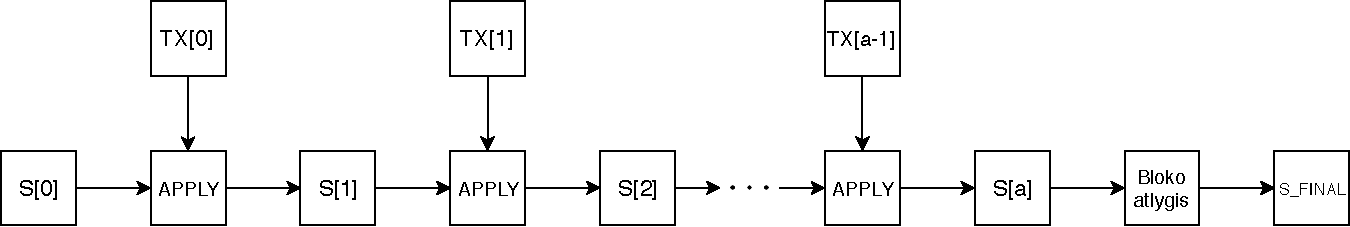
\includegraphics[scale=0.70]{img/pav-eth-chain.pdf}
    \caption{Blokų grandinės veikimo modelis \cite{buterin2014next}}
    \label{img:pav-block-chain}
\end{figure}

\subsubsection{Ethereum paskyra}
Ethereum platformoje būsena sudaryta iš objektų, vadinamų paskyromis (angl. \textit{Accounts}), kurių adresas yra 20 baitų ilgio, o būsenų pasikeitimais tampa tiesioginiai vertės ir informacijos apsikeitimai tarp paskyrų. Ethereum paskyra turi šiuos laukus \cite{buterin2014next}:
\begin{itemize}
    \item Skaitinė reikšmė, kuri užtikrina, kad transakcija gali būti įvykdoma tik kartą. 
    \item Esamas kriptovaliutos ether kiekis paskyroje. 
    \item Kontrakto programainis kodas (jei toks yra numatytas).
    \item Paskyros saugykla. Numatytoji saugyklos reikšmė yra tuščia.
\end{itemize}

Egzistuoja du paskyrų tipai: išoriškai valdomos paskyros ir išmaniųjų kontraktų paskyros. Išoriškai valdomą paskyrą gali valdyti tik tas, kas turi privatų paskyros raktą. Tuo tarpu išmaniojo kontrakto paskyra visiškai priklauso nuo jos programinio kodo.

\subsubsection{Žinutės ir transakcijos}
Žodis \textit{Transakcija} Ethereum kontekste reiškia pasirašytą duomenų paketą, talpinantį savyje žinutę, kuri būna inicijuojama išoriškai valdomos paskyros. Transakciją sudaro \cite{buterin2014next}:
\begin{itemize}
    \item Žinutės gavėjo adresas.
    \item Parašas, leidžiantis nustatyti siuntėjo identitetą.
    \item Kriptovaliutos ether kiekis, kurį siuntėjas perleidžia gavėjui.
    \item Neprivalomas duomenų laukas, paprastai leidžiantis siuntėjui aprašyti paskirtį arba kitas norimas transakcijos detales.
    \item Kintamasis STARTGAS. Tai reikšmė, nurodanti didžiausią kiekį skaičiavimo žingsnių, kuriuos vykdoma transakcija gali atlikti.
    \item Kintamasis GASPRICE. Tai reikšmė, nurodanti mokestį kriptovaliutos ether pavidalu, sumokamą už vieną skaičiavimo žingsnį.
\end{itemize}

Pirmosios trys reikšmės turėtų logiškai egzistuoti bet kokioje kriptovaliutos siuntimo architektūroje, kadangi tai yra fundamentalios sąvokos, reikalingos įvykdyti bet kokią transakciją. Tuo tarpu paskutinės dvi reikšmės STARTGAS ir GASPRICE yra Ethereum platformos architektūrinis sprendimas. 

Išmanieji kontraktai turi galimybę siųsti žinutes kitiems kontraktams. Žinutės yra virtualūs objektai, kurie nėra nuoseklinti (angl. \textit{Serialized}) ir egzistuoja tik Ethereum vykdymo aplinkoje. Žinutę sudaro \cite{buterin2014next}:
\begin{itemize}
    \item Žinutės siuntėjas.
    \item Žinutės gavėjas.
    \item Kriptovaliutos ether kiekis, kuris bus persiunčiamas kartu su žinute.
    \item Neprivalomas duomenų laukas.
    \item Kintamasis STARTGAS.
\end{itemize}

Iš esmės žinutė yra ne kas kita kaip transakcija, tik šiuo atveju inicijuojama ne išoriškai valdomos paskyros, o išmaniojo kontrakto.

\subsubsection{Kuras}
Visas blokų grandinės tinklas veikia internete ir naudoja elektros energiją, todėl nenuostabu, kad atlikus transakciją ir kitiems tinklo naudotojams ją patvirtinus, yra naudojama elektros energija, kuri kainuoja pinigus. Dėl šios priežasties buvo įvestas terminas \textit{kuras} (angl. \textit{Gas}). Šis kuras yra metafora realaus pasaulio kuro atitikmeniui, kuris leidžia naudotis paslaugomis ir patogumais. 

Kuro veikimo principas yra tarsi saugiklis, apsaugantis nuo skaičiavimo švaistymo programiniame kode bei neleidžiantis, kad įvyktų netyčiniai arba tyčiniai amžinieji ciklai, kurie galėtų iššvaistyti visas paskyros kriptovaliutos atsargas. Tam mes įvedame skaičiavimo žingsnių limitą STARTGAS. Jeigu transakcija pavyko sėkmingai, visas likęs kuras yra grąžinamas transakcijos iniciatoriui. Jeigu transakcijos kuras baigiasi dar prieš galutinai įvykdžius transakciją, visi transakcijos metu atlikti veiksmai yra anuliuojami, todėl transakcijos iniciatorius patiria nuostolius – už nurodytą STARTGAS sumokėti ether nėra grąžinami \cite{fekkes2018comparing}.

Siekiant suskaičiuoti, koks turėtų būti STARTGAS, į visumą reikia apimti daug kintamųjų. Paprastai vienos skaičiavimo operacijos kaina yra 1 kuro vienetas, tačiau yra operacijų, kainuojančių ir daugiau kuro vienetų, priklausomai nuo operacijos sudėtingumo ir naudojamos atminties. Taip pat yra 5 kuro vienetų kaina už kiekvieną transakcijos duomenų baitą. Taip pat reikia turėti omenyje, kad kintamojo GASPRICE kaina turėtų būti pakankamai konkurencinga ir ne per žema, nes Ethereum tinklo nariai, patvirtinantys transakcijas, gauna už tai atlygį kuro pavidalu, todėl jei nurodytas atlygis už transakcijos patvirtinimą bus mažesnis, nei visų kitų transakcijų tinkle, kyla rizika, kad transakcijos niekas taip ir nepatvirtins. 

Ši sistema apsaugo nuo piktavalių, kurių tikslas yra apkrauti Ethereum tinklą. Taigi, jei šių piktavalių tikslas būtų apkrauti visą Ethereum tinklą didžiuliais kiekiais skaičiavimų, jie turėtų turėti milžinišką kiekį kriptovaliutos, kurią įsigyti kainuotų labai didelius pinigus ir tikriausiai to įgyvendinimas būtų labai nuostolingas.

\subsubsection{Ethereum išmanieji kontraktai}
Išmanieji kontraktai Ethereum platformoje yra programinio kodo pavidalo, suprogramuoti aukšto lygio kalbomis. Tuomet šis kodas yra sukompiliuojamas į EVM baitinę programą (angl. \textit{Bytecode}), kuri patalpinama į Ethereum blokų grandinę vykdymui \cite{hildenbrandt2017kevm}. Ethereum naudoja aukšto lygio programavimo kalbą \textit{Solidity}, reikalingą suprogramuoti išmaniuosius kontraktus. Nors ir gali pasirodyti, kad programuotojai yra suvaržomi viena programavimo kalba, kurią reikia gerai išmanyti, norint parašyti aukštos kokybės kontraktus be klaidų, tačiau specialistai teigia, kad mokant kitas programavimo kalbas Solidity yra greitai išmokstama.

\subsubsection{Kitos Ethereum charakteristikos}
Ethereum technologija turi ir daugiau unikalių savybių, kurios išskiria šią platformą iš kitų. Aptarsime svarbiausias charakteristikas.

\subsubsubsection{Konsensuso mechanizmas}
Konsensuso mechanizmas blokų grandinės kontekste – tai bendras susitarimas, procesas, reikalingas tam, kad būtų pasiektas bendras sutarimas dėl duomenų tinkamumo ir patikimumo tarp skirtingų tinklo dalyvių. Ethereum šiuo metu naudoja įdėto darbo įrodymo konsensusą, reikalingą patvirtinti naujiems blokams.

PoW esmė – visi tinklo nariai atlieka mašininį skaičiavimo darbą sprendžiant tam tikras užduotis, o radęs sprendimą jį paskelbia visiems tinklo nariams, jeigu to jau nepadarė kas nors kitas. Jeigu sprendimas teisingas, šį atsakymą pateikęs asmuo gauna atlygį kriptovaliutos ether pavidalu, o naujas blokas yra prisegamas prie blokų grandinės galo. Sprendžiamos užduoties sudėtingumas yra labai aukštas, tačiau kitiems tinklo nariams patikrinti, ar užduoties sprendimas yra teisingas, turint atsakymą, yra labai lengva.

Šitaip atsiranda kriptovaliutų kasėjų (angl. \textit{Miners}) terminas. Šie kasėjai konkuruoja spręsdami užduotis, o pirmas teisingai išsprendęs tokią užduotį yra apdovanojamas kriptovaliuta ether. Tačiau šios užduotys yra be galo sudėtingos ir reikalauja milžiniškų elektros ir skaičiavimo galios išteklių, todėl paprastai kasėjai susivienija į grupuotes, kuriose kasimu užsiiminėja ne po vieną, o kaip bendra grupė \cite{bano2017consensus}. Šių grupių dydis gali siekti nuo keliolikos asmenų iki dešimčių tūkstančių, tačiau kuo daugiau narių, tuo labiau atlygio procentinė dalis sumažėja. 

Vienas pagrindinių PoW trūkumų – žala aplinkai, nes bendra kasimo metu suvartojama elektros energija viršija net kai kurių valstybių elektros suvartojimą, o ir pati kasimo galia tampa monopolizuojama. Tai paskatino Ethereum technologijos kūrėjus likti neabejingus ir ieškoti būdų keisti konsensuso mechanizmą. Tarp ateities planų yra numatomas turimų akcijų įrodymo konsensuso (angl. \textit{Proof of Stake – PoS}) įgyvendinimas, pavadinimu \textit{Casper}, kuris pašalins blokų kasimą atliekant skaičiavimus ir tinklas taps labiau saugus ir efektyvus \cite{buterin2017casper}.

\subsubsubsection{Blokų patvirtinimas}
Bloko patvirtinimo laikas šiuo metu yra apie 15 sekundžių \cite{park2017block}, o blokų kiekio patvirtinimas yra 12. Tai reiškia, jog tam, kad bloką galėtume pavadinti tikrai saugiu, po einamojo bloko turi sekti dar 12 blokų \cite{ekparinya2018double}. Taigi pilnas bloko patvirtinimo ciklas užtrunka apie 3 minutes (12 blokų po 15 sekundžių). 

Tokia blokų patvirtinimo sistema tinklo nariams leidžia apsisaugoti nuo kenkėjų: norint pakeisti giliau esančių blokų turinį, įsilaužėlis turės pats vienas sugeneruoti visus 12 tolimesnių blokų greičiau nei bet kas kitas tinkle. Kadangi blokų grandinė išsišakoja esant neatitikimams, galiausiai yra pasirenkama ilgiausia grandis, o trumpesnė atmetama \cite{bano2017consensus}. Taigi, esant PoW principui, vienam ar keliems naudotojams apgauti tinklą yra praktiškai neįmanoma.

\subsubsubsection{Transakcijų patvirtinimas}
Šiuo metu Ethereum palaiko apie 15 transakcijų per sekundę (TPS) \cite{park2017block}. Šis skaičius labai apriboja Ethereum platformą, nes jei kriptovaliuta ether pakeistų įprastas valiutas, iškiltų didžiulė problema – Ethereum tinklas taip sulėtėtų, kad atsiskaitymas už kasdienes prekes taptų neįmanomas. Be to, už kiekvieną apsipirkimą ir atliktą mokėjimą reikėtų sumokėti ir brangų transakcijų mokestį. 

Ethereum kūrėjai ieškojo sprendimų ir šiuo metu siekia pritaikyti į žaibišką tinklą (angl. \textit{Lightning Network}) \cite{poon2016bitcoin} panašią technologiją – Plazmą (angl. \textit{Plasma}). Šis tinklas leidžia atidaryti mokėjimo kanalą tarp 2 šalių ir neribotai atlikinėti transakcijas už blokų grandinės ribų. Uždarius šį kanalą, galutinis rezultatas yra įrašomas į blokų grandinę: kiekvienos šalies paskyros būsena, t.y. kriptovaliutos likutis \cite{poon2017plasma}. Dar viena naudinga Plazmos savybė – jei 2 šalys turi atsidariusios kanalą tarpusavyje, galima atsidaryti savo kanalą su viena iš šalių ir šitaip atlikinėti transakcijas tarp abiejų šalių.

\subsubsubsection{Kriptovaliutos išdavimas}
Šiuo metu rinkoje yra apie 100 milijonų kriptovaliutos Ether vienetų\footnote{https://coinmarketcap.com. Tikrinta 2018-06-17}, tačiau šis skaičius nuolat kinta dėl infliacijos. Kiptovaliutos infliacija nėra fiksuota, kadangi su kiekvienu pridedamu bloku yra sukuriami 5 ETH kriptovaliutos vienetai. Taigi, galima sakyti, kad metinė infliacija yra sparčiai mažėjanti.

\subsubsection{Pritaikymas}
Kadangi Ethereum į blokų grandinės rinką atėjo pakankamai anksti, kol dar nebuvo konkurencijos, ši platforma spėjo sulaukti didelio palankumo ir pripažinimo tarp programuotojų, kurie pasinaudojo pilnai veikiančia platforma, kad galėtų suskurti pirmuosius DApp. Šiuo metu yra užfiksuota apie pusantro tūkstančio tokių decentralizuotų programėlių\footnote{https://www.stateofthedapps.com/rankings. Tikrinta 2018-06-17}. Visus projektus būtų galima skirstyti į 2 kategorijas:  \begin{itemize}
    \item Finansiniai projektai. Tai draudimo paslaugų, taupomųjų piniginių, testamentų, įdarbinimo sutarčių, duomenų saugojimo aplikacijos.
    \item Projektai, visiškai nesusiję su finansais. Tai internetinio balsavimo, decentralizuoto valdymo, medicinos sistemos.
\end{itemize}

\clearpage

\subsection{EOS išmaniųjų kontraktų platforma}
Kaip teigia patys technologijos kūrėjai, EOS yra pati galingiausia infrastruktūra decentralizuotų aplikacijų kūrimui, o dauguma blokų grandinės technologijos entuziastų tikina, kad būtent EOS bus vienas didžiausių Ethereum konkurentų rinkoje ar net vadina jį Ethereum žudiku. EOS žada operacinės sistemos pobūdžio įrankius ir paslaugas decentralizuotų aplikacijų kūrimui, prieglobai (angl. \textit{Hosting}) ir vykdymui. Tiesa, ne visos savybės ir funkcionalumas, aprašytas sekančiai yra įgyvendintas – EOS pradėjo vysytis 2017 metais ir kūrėjai įgyvendina technologiją palaipsniui pagal planą, tačiau šiame darbe bus nagrinėjama visuma darant prielaidą, jog technologija yra iki galo užbaigta, kaip suplanuota.

\subsubsection{EOS kriptovaliuta}
Iki 2018 metų birželio 1 dienos EOS kriptovaliuta egzistavo Ethereum blokų grandinėje ERC20 žetonų forma. Tačiau atėjus šiam terminui visi ERC20 žetonai buvo užšaldyti, o visų savininkų EOS žetonai perkelti į pagrindinį EOS tinklą (angl. \textit{Mainnet}) kriptovaliutos EOS pavidalu. 

Šios kriptovaliutos viena iš paskirčių – decentralizuotų aplikacijų kūrėjams suteikti galimybę kurti savo žetonus, pritaikytus jų aplikacijų platformoms. Tačiau ko gero dar įdomesnė kriptovaliutos EOS savybė – pralaidumo (angl. \textit{Bandwidth}) ir talpyklos valdymas blokų grandinėje. Pavyzdžiui, asmuo, turintis 1\% visų EOS kriptovaliutos vienetų, gali valdyti iki 1\% viso EOS blokų grandinės pralaidumo. Kriptovaliutos turėjimas suteikia visos blokų krandinės akcininko rolę, kuri leidžia proporcingai pagal turimą kriptovaliutos kiekį dalyvauti balsavimuose ir sprendimų priėmime \cite{Cox2018next}.

\subsubsection{EOS žetonai}
Kaip ir Ethereum, EOS turi savo žetonų standartą, kurį aprašo žetonų interfeisas. Šis interfeisas nurodo tokias funkcijas, kurias reikia įgyvendinti, norint sukurti savo žetonus \cite{Cox2018next}:
\begin{itemize}
    \item Sukurti Z tipo žetonus, nustatant jų maksimalų kiekį N.
    \item Išduoti N žetonų paskyrai X.
    \item Pervesti N žetonų iš paskyros X į paskyrą Y.
    \item Sužinoti visą Z žetonų tipo kiekį.
    \item Sužinoti sąskaitos X turimų žetonų skaičių.
\end{itemize}

\subsubsection{Virtuali mašina}
EOS bus vienintelė platforma, kuri taikys autorizuotas žinutes kitoms paskyroms, vadinamas veiksmais (angl. \textit{Actions}). EOS nesiūlo savo unikalios virtualiosios mašinos. Vietoje to, bet kokia kalba ar virtualioji mašina, kuri yra deterministinė, tinkamai uždara ir turinti pakankamą našumą, galės būti integruota kartu su EOS programinės įrangos API sąsaja. Skriptų kalbos ir virtualios mašinos detalės tėra specifinės įgyvendinimo detalės, kurios nepriklauso nuo EOS technologijos. 

Visi paskyrų tarpusavio veiksmų siuntinėjimai yra apibrėžti schemos. Ši schema įgalina sklandų komunikavimą tarp JSON ir dvejetainių veiksmų formatų. Duomenų bazės būsena taip pat yra apibrėžta panašios schemos. Tai užtikrina, kad visi duomenys, saugomi programose, yra tokio formato, kuris gali būti interpretuojamas kaip JSON, bet saugomas ir manipuliuojamas tokiu efektyvumu, kaip dvejetainis kodas.

\subsubsection{EOS paskyra}
EOS paskyra yra tam tikras identifikatorius, saugomas blokų grandinėje. Kiekvienai transakcijai suteikiami leidimai, nustatomi pagal paskyros įgaliojimų konfigūraciją. Paskyra gali priklausyti asmeniui arba asmenų grupei, priklausomai nuo įgaliojimų konfigūracijos. Kiekviena paskyra turi 2 numatytas įgaliojimų rūšis \cite{Cox2018next}:
\begin{itemize}
    \item \textbf{Savininko įgaliojimai} (angl. \textit{Owner}). Šie įgaliojimai parodo, kas yra teisėtas paskyros savininkas. Yra keletas transakcijų, kurios reikalauja šių įgaliojimų, tačiau jos yra svarbiausios, nes yra susijusios su bet kokiu paskyros nuosavybės pasikeitimu. Yra siūloma, kad įrodymai apie savininko įgaliojimus būtų saugomi labai atsargiai ir apie juos žinotų tik tikrasis paskyros savininkas.
    \item \textbf{Aktyvūs įgaliojimai} (angl. \textit{Active}), kurie leidžia persiųsti paskyros turimas lėšas, leisti atlikti balsavimus sprendžiant blokų gamintojus ir kitas aukšto lygio paskyros manipuliacijas.
\end{itemize}
Verta paminėti, kad įgaliojimai čia nesibaigia ir programuotojai gali kurti savo specifinius įgaliojimus, kurie gali būti reikalingi įvairiems panaudos atvejams ir paskyros valdymo praplėtimui.

Taip pat EOS paskyras gali valdyti daugiau nei vienas asmuo. Tokiu atveju veiksmus, reikalaujančius savininko įgaliojimų, turi patvirtinti visi savininkai su savo privačiais raktais, o norint atlikti veiksmus, reikalaujančius aktyvių įgaliojimų, pakanka tik vieno iš savininkų patvirtinimo.

Dar viena EOS paskyros savybė – paskyros savininkas gali suteikti leidimą naudotis paskyra ir veikti savininko vardu nesuteikiant pilnos paskyros valdymo teisės. Tokiu atveju įgaliotasis asmuo turėtų naudoti savo privatų raktą padėdamas parašą ant atliekamų veiksmų autorizacijos metu. Tai leistų paskyros savininkui atsekti kas ir kokiais būdais naudojosi paskyra, tarsi matydamas visų veiksmų žurnalą.

\subsubsection{Transakcijos ir veiksmai}
Veiksmas (angl. \textit{Action}) EOS kontekste reiškia vieną operaciją, kai tuo tarpu transakcija yra vieno arba daugiau veiksmų rinkinys. Veiksmai gali būti siunčiami atskirai po vieną, arba siunčiami kaip visuma, jeigu juos norima interpretuoti kaip atominį vienetą. Pateikiama pavyzdinė transakcijos struktūra su vienu veiksmu JSON formatu (žr. Priedas nr. 3).

Labai svarbi transakcijų savybė yra ta, kad vykdyti transakcijas galima be jokio mokesčio. Jeigu asmeniui priklauso 1\% visos EOS kriptovaliutos, tai reiškia, kad jis valdo iki 1\% resursų visame EOS tinkle. Todėl jei šis savininkas neatlieka daugiau transakcijų ir neapkrauna tinklo didesniu nei 1\% duomenų srautu, naudojimasis EOS technologija jam nieko nekainuos. Tačiau EOS atveria ir daugiau galimybių – resursus įmanoma nuomoti. Tai leis decentralizuotų aplikacijų kūrėjams ir kitoms suinteresuotoms šalims, kurie neturi pakankamai EOS resursų, nuomotis juos iš tų, kurie pilnai neišnaudoja savo turimų išteklių.

\subsubsection{EOS išmanieji kontaktai}
EOS išmaniųjų kontraktų programuotojai, priešingai nuo Ethereum, nebus suvaržyti viena programavimo kalba. EOS išmaniuosius kontraktus galima programuoti visomis programavimo kalbomis, kurios gali būti sukompiliuotos į tinklo asemblerį (angl. \textit{Web Assembly}) – WASM. Tai reiškia, kad programuotojams atsiranda laisvė rinktis tarp tokių kalbų, kaip C++, C, Rust ir kitomis, kurios sparčiai tampa pritaikomos suderinamumui su WASM.

\subsubsection{Kitos EOS charakteristikos}
Toliau pateikiamos kitos EOS platformos savybės ir detalės, turinčios konkurencinę prasmę blokų grandinės rinkoje.

\subsubsubsection{Konsensuso mechanizmas}
Priešingai nei Ethereum, EOS naudoja dedikuotą turimų akcijų įrodymo konsensusą (angl. \textit{Delegated Proof of Stake}) – DPoS. Naudojant DPoS protokolą, visi kriptovaliutos EOS savininkai gali balsuoti už deleguotus atstovus – blokų gamintojus (angl. \textit{Block Producer}), kurie yra atsakingi už transakcijų bei naujų blokų patvirtinimą \cite{DPoS2018feat}. Pretenduoti tapti delegatu gali visi, tačiau tik 21 delegatai, surinkę daugiausiai balsų galės tapti blokų gamintojais. Konkurencija tapti blokų gamintojų bus labai didelė, kadangi už transakcijų patvirtinimą ir pridėjimą prie blokų grandinės yra gaunamas atlygis. 

Tokia sistema taip pat padidina saugumą ir grandinės patikimumą, kadangi blokų gamintojai norės būti patikimais delegatais – maždaug kas 63 sekundes vyks delegatų perrinkimas, todėl jei delegatas pasirodys nepatikimas, darantis klaidas arba atstovaujantis savo, o ne tinklo narių interesus, greičiausiai jis nebus išrinktas dar kartą.

\subsubsubsection{Lygiagretusis vykdymas}
Viena išskirtinė savybė, kuria EOS siekia efektyvinti savo tinklą – tai lygiagretusis vykdymas. Ši savybė leistų vienu metu tiek vykdyti išmaniuosius kontraktus, tiek apdoroti transakcijas. Iki šiol abu veiksmus buvo galima atlikti tik nuosekliai, o įgyvendinus lygiagretųjį vykdymą transakcijas būtų galima apdoroti lygiagrečiai \cite{vukolic2015quest}. Vienas to pavyzdys – veiksmai, kurie yra įtraukti į transakcijas, tačiau nepriklauso nuo blokų grandinės būsenos, todėl jie gali būti pilnai vykdomi lygiagrečiai, o tai potencialiai reikštų net milijoninius TPS rodiklius.

\subsubsubsection{Blokų grandinių tarpusavio komunikavimas}
Blokų grandinių tarpusavio komunikavimas (angl. \textit{Inter-Blockchain Communication}) – tai dar viena artimiausiu metu planuojama įgyvendinti EOS savybė, aprašyta \cite{chen2017inter}. Šis būdas leidžia patikimu ir saugiu būdu patikrinti, ar įvykis yra autentiškas kitoje blokų grandinėje. EOS kontekste tai reiškia realizuoti lengvojo kliento programą (angl. \textit{Light Client}) kaip išmanųjį kontraktą. Lengvojo kliento programa sugeba patvirtinti blokų grandinės transakcijas, neapdorojant visos blokų grandinės.

\subsubsubsection{Blokų patvirtinimas}
EOS blokus gamina raundais po 126 blokus (kiekvienam iš 21 blokų gamintojų tenka po 6 blokų patvirtinimus) \cite{Cox2018next}. Kiekvienas blokas yra patvirtinamas per 0,5 sekundės – tai labai suspartina decentralizuotų programėlių reakcijos laiką. Tam, kad blokas taptų nepakeičiamas ir įrašytas į blokų grandinę visam laikui, reikia kvalifikuotos blokų gamintojų daugumos – daugiau nei 2/3 visų blokų gamintojų – 15 uždėtų parašų ant bloko, patvirtinančių bendrą blokų gamintojų sutikimą dėl bloko tinkamumo.

\subsubsubsection{Transakcijų patvirtinimas}
Patvirtinamų transakcijų kiekis per sekundę yra pakankamai nepastovus kriterijus. Viena iš to priežasčių – skirtingos konfigūracijos ir optimizavimo metodai. Blogiausiu atveju EOS galėtų aptarnauti 1000 TPS, o geriausiu – 6000 TPS.

Kaip jau žinome, transakcijos EOS tinkle yra praktiškai nemokamos, tad kaip užsidirba išrinkti blokų gamintojai? Atsakymas yra infliacija. Kiekvienas blokų gamintojas gaus dalį EOS kriptovaliutos nuo metinės infliacijos priklausomai nuo jį išrinkusių vartotojų balsų dalies.

\subsubsubsection{Kriptovaliutos išdavimas}
Šiuo metu visoje kriptovaliutų rinkole yra išduota beveik milijardas EOS kriptovaliutos vienetų, išdalintų EOS ICO metu. Tačiau tai nėra šios kriptovaliutos limitas, kadangi yra numatyta iki 5\% kasmetinės infliacijos. Ši infliacija yra sukurta tam, kad ateityje būtų išvengta kriptovaliutos deficito, nes tikimasi didelio jos paklausos augimo kuriant įvairias programėles tinkle.

\subsubsection{Pritaikymas}
Deja, bet šiuo metu nėra nė vienos veikiančios decentralizuotos aplikacijos EOS platformoje, tačiau tik dėl to, kad pagrindinis EOS tinklas dar neįsigalėjo. Todėl, kai birželį bus paleistas EOS pagrindinis tinklas ir bus aišku dėl stabilaus jo veikimo, startuos didesni projektai, tokie kaip Everipedia, Scatter, Billionaire Token ir kiti\footnote{https://eosforum.org/t/eos-dapp-collection-28-listed-currently. Tikrinta 2018-06-17}.

\clearpage

\subsection{Ethereum ir EOS išmaniųjų kontraktų platformų palyginimas}

Šiame skyriuje apibendrinamos ir palyginamos Ethereum ir EOS išmaniųjų kontraktų platformų svarbiausios savybės, ypatumai ir detalės, turinčios reikšmę išmaniųjų kontraktų kūrimo procese arba prieš nusprendžiant kurti išmaniuosius kontraktus.

{\centering

\begin{longtable}{|L{3,8cm}|L{5,3cm}|L{6cm}|}
\caption{Ehereum ir EOS palyginimas}
\label{variability_impl_mech}
\endfirsthead
\endhead
\hline

\textbf{Palyginimo kriterijus} & \multicolumn{1}{c|}{\textbf{Ethereum}} & \multicolumn{1}{c|}{\textbf{EOS}} \\ \hline

\textbf{Kriptovaliuta} & Ether & EOS \\ \hline

\textbf{Kriptovaliutos paskirtis}     
& Apmokėti kompiuterinių skaičiavimų sąnaudas ir transakcijų mokesčius & Decentralizuotų aplikacijų žetonų kūrimas, EOS tinklo resursų valdymas, EOS akcininko rolės vaidmuo balsavime \\ \hline

\textbf{Kriptovaliutos išdavimas} & \textasciitilde100 milijonų ETH & ~900 milijonų EOS \\ \hline

\textbf{Kriptovaliutos metinė infliacija} & Mažėjanti – į rinką išleidžiamas apytikriai tas pats kriptovaliutos kiekis per metus & Fiksuota – iki 5\% infliacijos \\ \hline

\textbf{Kriptovaliutos žetonai} & Neprivalomas įgyvendinti ERC20 standartinis interfeisas su 6 metodais & Kuriant žetonus būtina įgyvendinti žetono interfeisą su 5 metodais \\ \hline

\textbf{Vykdymo aplinka, virtuali mašina}   & Tiuringo mašiną atitinkanti EVM, priimanti ir vykdanti išmaniųjų kontraktų baitinį kodą. EVM kodą vykdo kiekvienas tinklo narys & Neturi virtualiosios mašinos, labiau atitinka operacinės sistemos paskirtį. Kitos platformos bei virtualiosios mašinos gali būti integruojamos su EOS API \\ \hline

\textbf{Lygiagretusis vykdymas} & Nepalaikomas & Ateityje siekiama įgyvendinti \\ \hline

\textbf{Blokų grandinių tarpusavio komunikavimas} & Nepalaikomas & Ateityje siekiama įgyvendinti \\ \hline

\textbf{Plazma} & Ateityje siekiama įgyvendinti & Nepalaikomas \\ \hline

\textbf{Išmanieji kontraktai} & Naudojama Solidity programavimo kalba & Naudojamos programavimo kalbos, sukompiliuojamos į WASM: C++, C, Rust ir kitos \\ \hline

%\textbf{Platformos suteikiamas papildomas funkcionalumas} & Tikslingi vengiama funkcionalumo & Suteikiamas papildomas funkcionalumas \\ \hline

\textbf{Paskyra}  & Palaikomas vieno savininko funkcionalumas & Palaikomas daugelio savininkų funkcionalumas, suteikiama galimybė suteikti įgaliojimus naudotis paskyra, nuomoti resursus \\ \hline

\textbf{Transakcijos} & Transakcijos standartas su unikaliais STARTGAS ir GASPRICE laukais & Specialus EOS transakcijos standartas. Transakcijos gali turėti specialius autorizuotus veiksmus \\ \hline

\textbf{Transakcijų mokęstis} & Apskaičiuojamas pagal specialią formulę naudojant STARTGAS ir GASPRICE laukus & Disponuojant tam tikru kiekiu EOS kriptovaliutos, transakcijos tampa nemokamos \\ \hline

\textbf{Transakcijų patvirtinimas} & \textasciitilde15 TPS & 1000-6000 TPS \\ \hline

\textbf{Konsensuso mechanizmas} & PoW konsensusas. Planuojama pereiti prie PoS & DPoS konsensusas. \\ \hline

\textbf{Blokų patvirtinimas} & Bloką gali tvirtinti bet kuris tinklo narys. Blokas laikomas saugiu, jei po jo seka 12 patvirtintų blokų. Vieno bloko patvirtinimas užtrunka 15 sekundžių & Blokus patvirtina 21 išrenkamas blokų gamintojas raundais po 126 blokus. Blokas laikomas saugiu patvirtinus bloką kvalifikuota balsų dauguma. Vieno bloko patvirtinimas užtrunka 0,5 sekundės \\ \hline

\textbf{Pritaikymas} & Keli tūkstančiai projektų sukurtų ir veikiančių Ethereum platformoje & Kol kas nėra veikiančių decentralizuotų aplikacijų pagrindiniame EOS tinkle \\ \hline
\end{longtable}}

\sectionnonum{Rezultatai ir išvados}
Šiame darbe pavyko pasiekti tokius rezultatus:
\begin{enumerate}
    \item Išsiaiškinta blokų grandinės ir išmaniųjų kontraktų esmė: charakteristikos, veikimo principo detales bei svarbiausios sąvokos.
    \item Apžvelgta Ethereum išmaniųjų kontraktų platforma: blokų grandinės, kriptovaliutos ir išmaniųjų kontraktų specifika, transakcijų ir paskyrų samprata. Aptartos svarbiausios platformos charakteristikos ir pritaikymo paplitimas.
    \item Apžvelgta EOS išmaniųjų kontraktų platforma: blokų grandinės, kriptovaliutos ir išmaniųjų kontraktų specifika, transakcijų ir paskyrų samprata. Išnagrinėtos konkurencingiausios jos charakteristikos, planuojami atnaujinimai platformoje.
    \item Ištirti Ethereum ir EOS išmaniųjų kontraktų platformų skirtumai.
\end{enumerate}
\vspace{0.75\baselineskip}

Šiame darbe galėjome įsitikinti, kad blokų grandinės ir išmaniųjų kontraktų technologijos pasižymi unikaliomis savybėmis, kurias išvysčius, ateityje gali pakeisti interneto samprata, programų sistemų kūrimo įrankiai ir architektūra. Protingai kuriamos programėlės blokų grandinėse gali sukelti rimtą konkurenciją sistemoms, paremtoms tradiciniais modeliais. 

Atliktas tyrimas atskleidė, kad Ethereum platforma dėl savo ankstyvo įsitvirtinimo rinkoje vienareikšmiškai lenkia EOS pritaikymo srityje, tačiau yra verta konstruktyvios kritikos dėl kitų aspektų. Programų sistemų kūrėjai, prieš planuodami kurti sistemas Ethereum platformoje, privalo žinoti, kad tinklo galimybės yra ribotos – tinklas gali apdoroti tik kelioliką transakcijų per sekundę, o mokesčiai renkami net ir už smulkias operacijas tinkle. Tai reiškia, kad sistemų kūrėjai, dėl šių Ethereum savybių šiuo metu negali efektyviai realizuoti sudėtingų ir didelį naudotojų krūvį suvaldančių sistemų.

Tačiau, jeigu Ethereum kūrėjai realizuotų Casper protokolą ir Plazmos technologiją, minėtos problemos išsispręstų savaime. Plazma suteiktų labai daug lankstumo Ethereum platformai, nes būtų galima išvengti TPS lubų, o kartu ir mokesčių už kiekvieną operaciją. Tuo tarpu Casper padidintų viso Ethereum tinklo saugumą, efektyvumą ir decentralizaciją, nes PoW konsensusas būtų pakeistas į PoS mechanizmą.

Tyrimo metu atsiskleidė ne ką mažiau įspūdingesni EOS privalumai ir perspektyvos. Ateidami į rinką gana vėlai, EOS technologijos kūrėjai žinojo, kad turi pasiūlyti inovatoriškus sprendimus ir pasimokyti iš konkurentų klaidų. EOS jau dabar smarkiai lenkia Ethereum tokiais rodikliais, kaip transakcijų kiekis per sekundę ir mokesčiai už jas. Taip pat, priešingai nei Ethereum, EOS išmaniuosius kontraktus galima programuoti platesne ir labiau tradicine programavimo kalbų aibe, todėl tikėtina, kad programuotojams bus paprasčiau rašyti programinį kodą. 

Tiesa, to gali neužtekti konkuruojant su Ethereum, nes įgyvendinus Casper ir Plazmos technologiją, minėti pranašumai gali prarasti reikšmę. Ypač, kai EOS platformoje kol kas neegzistuoja veikiančių DApp pavyzdžių. Siūlomas akcininko rolės vaidmuo, patogesnis konsensuso mechanizmas, turimų resursų nuoma išskiria EOS tarp konkurentų, tačiau tik įgyvendinus lygiagretųjį vykdymą ir blokų grandinių tarpusavio komunikavimą būtų galima tvirtai kalbėti apie pokyčius programų sistemose.

Tuo tarpu Ethereum platformai būtų logiška pereiti prie panašaus konsensuso mechanizmo, kaip EOS, kuris sumažintų transakcijų mokesčius ir nereikalautų didelių elektros sąnaudų sėkmingam blokų grandinės tinklo funkcionavimui. Taip pat pradėti ieškoti lygiagretaus vykdymo galimybių, suderinamumo su kitomis blokų grandinėmis ir kitų platformos išplėtimo galimybių.

Šiame darbe galėjome įsitikinti, kad blokų grandinės technologija ir išmaniųjų kontraktų platformos dar labai jaunos ir joms reikia daugiau laiko naujų pritaikymų paieškai, kitų technologijų integravimui ir infrastruktūros gerinimui, todėl ateityje konkurencija šioje rinkoje turėtų tik aštrėti, o tuo pačiu tobulėti ir pati technologija. Pamatėme, kad išmaniųjų kontraktų platformos turi daug reikšmingų smulkių techninių detalių ir aspektų, galinčių daryti kritinę įtaką pačių išmaniųjų kontraktų prieinamumui, efektyvumui ir patogumui. Tačiau svarbiausi aspektai išlieka pradinis technologijos pamatas – tai yra decentralizacija ir saugumas.

\printbibliography[heading=bibintoc]

\sectionnonum{Sąvokų apibrėžimai}
\textbf{Bitkoinas} – pirmoji blokų grandinės kriptovaliuta.

\textbf{Blokų gamintojas} – blokų grandinės narys, išrinktas kitų blokų grandinės narių tam, kad patvirtintų blokus.

\textbf{Blokų grandinė} – nuolat augantis blokais sujungtas sąrašas, apsaugotas naudojant kriptografijos metodus.

\textbf{Decentralizuota programėlė} – programa, veikianti blokų grandinėje dažniausiai naudojant išmaniuosius kontraktus.

\textbf{Dedikuotas turimų akcijų įrodymas} – konsensuso mechanizmas, leidžiantis blokų grandinės tinklo nariams išrinkti blokų gamintojus.

\textbf{EOS} – išmaniųjų kontraktų platforma, pradėta vystyti 2017 metais. Taip pat EOS išmaniųjų kontraktų platformos kriptovaliutos pavadinimas.

\textbf{ERC20} – Ethereum platformos išmaniųjų kontraktų standartas, įgyvendinantis žetonų kūrimą.

\textbf{Ether} – Ethereum išmaniųjų kontraktų platformos kriptovaliutos pavadinimas.

\textbf{Ethereum} – viena pirmųjų išmaniųjų kontraktų platformų, pradėta vystyti 2014 metais. 

\textbf{Ethereum virtuali mašina} – virtuali vykdymo aplinka, įgalinanti išmaniųjų kontraktų paleidimą ir vykdymą.

\textbf{Išmanusis kontraktas} – protokolas arba programa, kuri įgyvendina automatinius skaitmeninės nuosavybės pervedimus tarp skirtingų šalių, remiantis bendrai sutartomis ir apibrėžtomis taisyklėmis.

\textbf{Įdėto darbo įrodymas} – konsensuso mechanizmas, parodantis, kad blokas buvo sukurtas įdedant didelę kompiuterinio skaičiavimo galią.

\textbf{Kriptovaliuta} – virtuali valiuta, kuria galima atsiskaitinėti blokų grandinėje išvengiant bankų sistemų.

\textbf{Kriptovaliutos piniginė} – adresas, turintis viešąjį raktą ir apsaugotas privačiu raktu, leidžiantis disponuoti turimomis kriptovaliutomis.

\textbf{Kriptovaliutų kasėjai} – blokų grandinės tinklo nariai, užsidirbantys iš PoW konsensuso gamindami blokus ir patvirtindami transakcijas.

\textbf{Kriptovaliutų keityklos} – internetiniai puslapiai arba programėlės, leidžiančios keisti vienas kriptovaliutas į kitas.

\textbf{Laiko žymė} – užfiksuotas laiko momentas.

\textbf{Lengvasis klientas} – blokų grandinės narys, galintis atlikti bazinių operacijų aibę blokų grandinėje naudojant minimalius resursus, tačiau negalintis atlikti sudėtingesnių, daugiau resursų reikalaujančių operacijų.

\textbf{Maišos reikšmė} – reikšmė, kurią apskaičiuoja maišos funkcija.

\textbf{Merkle medis} – medžiu paremta hierarchinė duomenų struktūra, kurioje kiekvienos vidinės viršūnės reikšmė yra tos viršūnės vaikų maišos reikšmė.

\textbf{Nuoseklinimas} – specifinių duomenų išsaugojimas į patogų nuskaityti ir saugoti formatą.

\textbf{Pirminis kriptovaliutos siūlymas} – kriptovaliutos siūlymas potencialiems jos naudotojams bei investuotojams mainais už pinigus suteikiant pažadą, kad kriptovaliutos kūrėjai sukurs atsiperkančią ir naudingą investuotojams sistemą.

\textbf{Plazma} – technologija, leidžianti atlikti didelį kiekį ir sparčias transakcijas už blokų grandinės ribų.

\textbf{Solidity} – išmaniųjų kontraktų kūrimui skirta programavimo kalba.

\textbf{Tinklo asembleris} – tinklo standartas, apibrėžiantis dvejetainį formatą ir analogišką asemblerio tipo tekstinį formatą kodo vykdymui internetiniuose puslapiuose.

\textbf{Turimų akcijų įrodymas} – konsensuso mechanizmas, kuriame bloko gamintojai yra parenkami pagal objektyvius kriterijus, pavyzdžiui atsitiktinai remiantis turimos kriptovaliutos kiekiu.

\textbf{Žetonas} – virtualus objektas, reikalingas naudojantis decentralizuotos programėlės paslaugomis.

\sectionnonum{Santrumpos}
\textbf{DApp} – decentralizuota programėlė.

\textbf{DPoS} – Dedikuotas turimų akcijų įrodymo konsensusas.

\textbf{ERC20} – išmaniųjų kontraktų standarto pavadinimas.

\textbf{ETH} – Ether.

\textbf{EVM} – Ethereum virtuali mašina.

\textbf{ICO} – Pirminis kriptovaliutų siūlymas (angl. \textit{Initial Coin Offering}).

\textbf{PoS} – Turimų akcijų įrodymo konsensusas (angl. \textit{Proof of Stake}).

\textbf{PoW} – Įdėto darbo įrodymas (angl. \textit{Proof of Work}).

\textbf{TPS} – Transakcijos per sekundę.

\textbf{WASM} – tinklo asembleris (angl. \textit{Web Assembly}).





\clearpage

\appendix 

\section{Standartinis verslo tinklo modelis}
\begin{figure}[H]
    \centering
    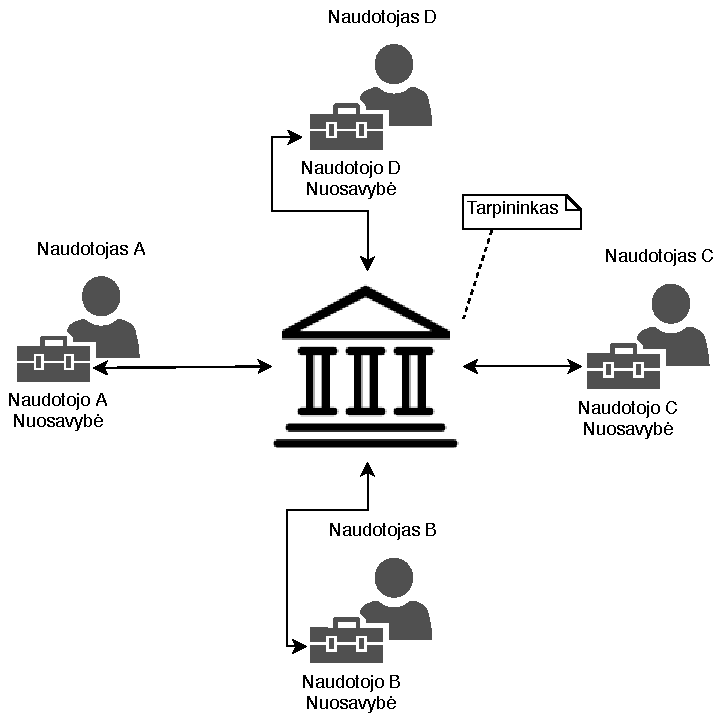
\includegraphics[scale=0.9]{img/pav-1.pdf}
    \caption{Standartinis verslo tinklo modelis}
    \label{img:pav-1}
\end{figure}

\section{Blokų grandinės verslo tinklo modelis}
\begin{figure}[H]
    \centering
    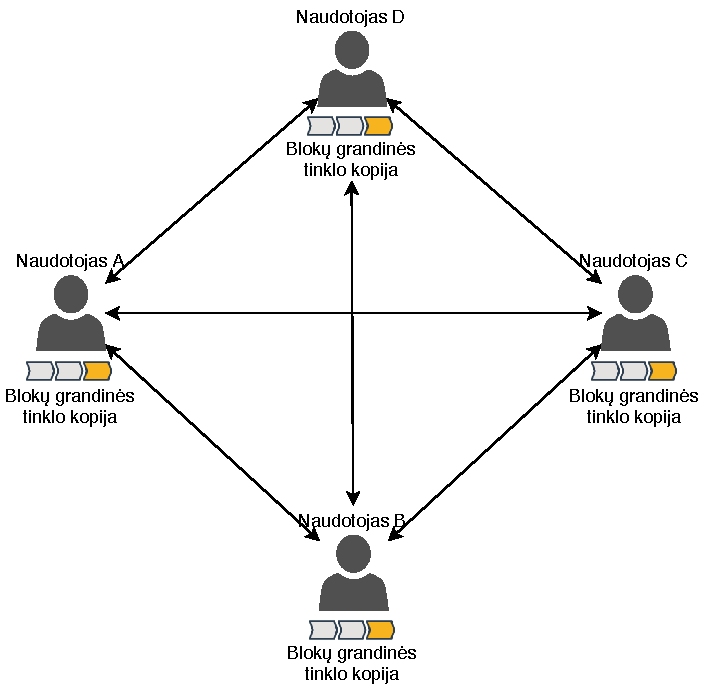
\includegraphics[scale=0.9]{img/pav-2.pdf}
    \caption{Blokų grandinės verslo tinklo modelis}
    \label{img:pav-2}
\end{figure}

\section{EOS išmaniųjų kontraktų transakcija su vienu veiksmu kodo fragmentas}
\begin{figure}[H]
    \centering
    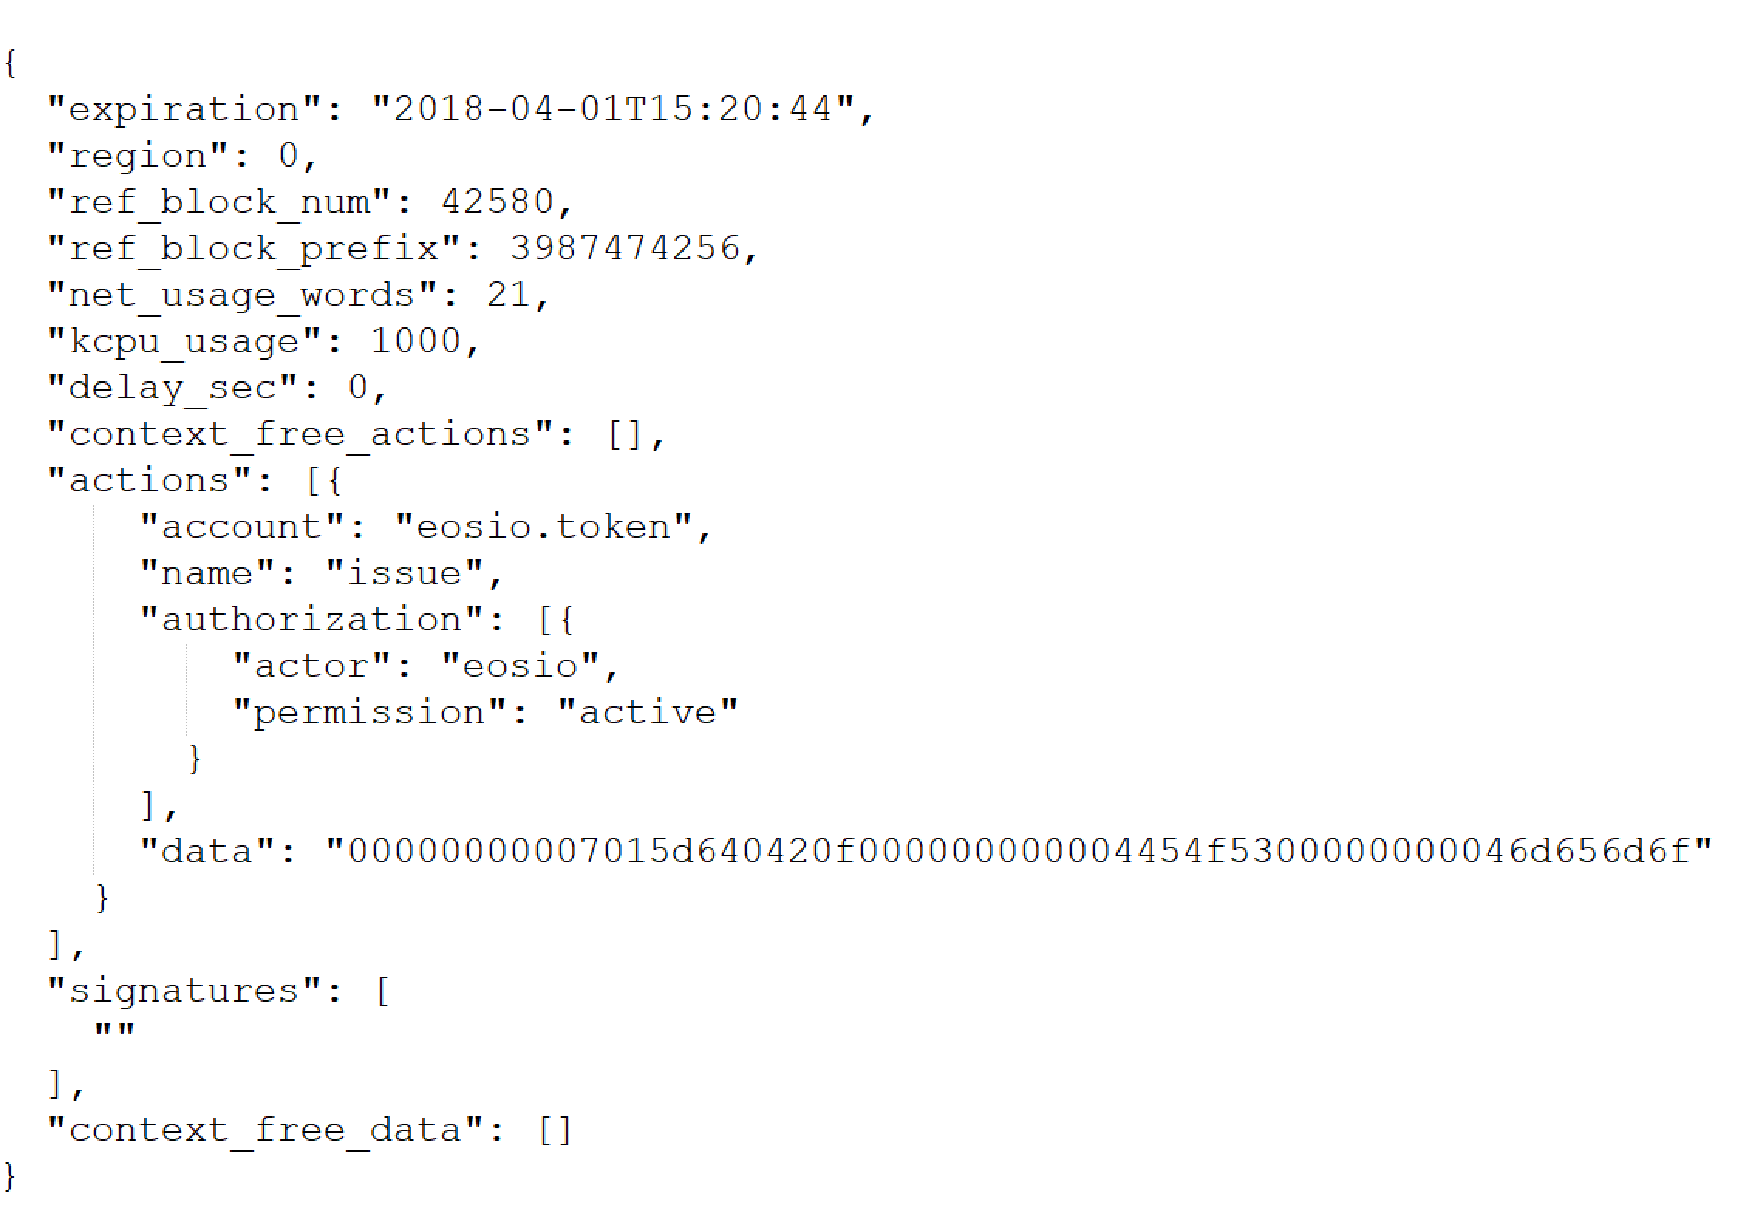
\includegraphics[scale=0.55]{img/pav-4.pdf}
    \caption{EOS transakcijos kodas JSON formatu}
    \label{img:pav-4}
\end{figure}

\end{document}
